\chapter{Prévision}

\section{Introduction}

Dans cette partie, nous tenterons de définir des propositions de pistes de recherche pour le mémoire. Nous commencerons par donner un bref aperçu du contexte relatif à la mobilité des véhicules à l'échelle des grandes villes. Nous continuerons par fournir une description d'un ensemble de données liées à cette mobilité. Et, nous terminerons par donner un plan et des idées de solutions pour ce genre de problématique.

\section{Contexte}

Ces dernières années, il est apparu un nombre important de tentatives de solutions aux problèmes de réseaux routiers liés à la mobilité véhiculaire. Seulement, l'essentiel de ces solutions ont été éprouvés par le biais de simulateurs puisque l'expérimentation étant pratiquement impossible pour des raisons pratiques et les approches analytiques étant souvent trop complexes. La justesse de la simulation étant d'autant plus capitale qu'il n'existe pas de jeu de données capturant à la fois les dynamiques microscopiques et macroscopiques des trajets~\cite{uppoor2014generation}.

De fait, l'évaluation des performances des réseaux routiers est souvent biaisé par la manière dont se déplacent les véhicules, ce qui affecte le protocole utilisé et donc le déplacement de ces voitures. Cette situation peut mener à des mauvaises conclusions si le trafic est représenté incorrectement, et ce, indépendamment de la simulation~\cite{bai2003important}.

On a alors cherché à améliorer les modèles représentant les déplacements des voitures, tout d'abord en employant des techniques stochastiques (\textit{Random Waypoint}), puis en tenant en compte des propriétés topologiques~\cite{saha2004modeling}. Ensuite, on a voulu inclure le comportement des véhicules au niveau microscopique ou encore la signalisation~\cite{harri2009mobility}. Pour aboutir au simulateur le plus poussé sur le marché, SUMO~\cite{SUMO2012}.

SUMO est un simulateur, libre de sources et de droits, dédié à la simulation de trafic urbain. Il permet de modéliser tant les véhicules ou les transports publiques que les piétons. En outre, il propose nativement une pléthore d'outils afin de visualiser les trajets, d'importer des cartes et des comportements ou encore de calculer les taux d'émission en particule. Il propose également une interface riche où peut se greffer facilement de nombreux autres outils~\cite{SUMO2012}.

\begin{figure}[ht]
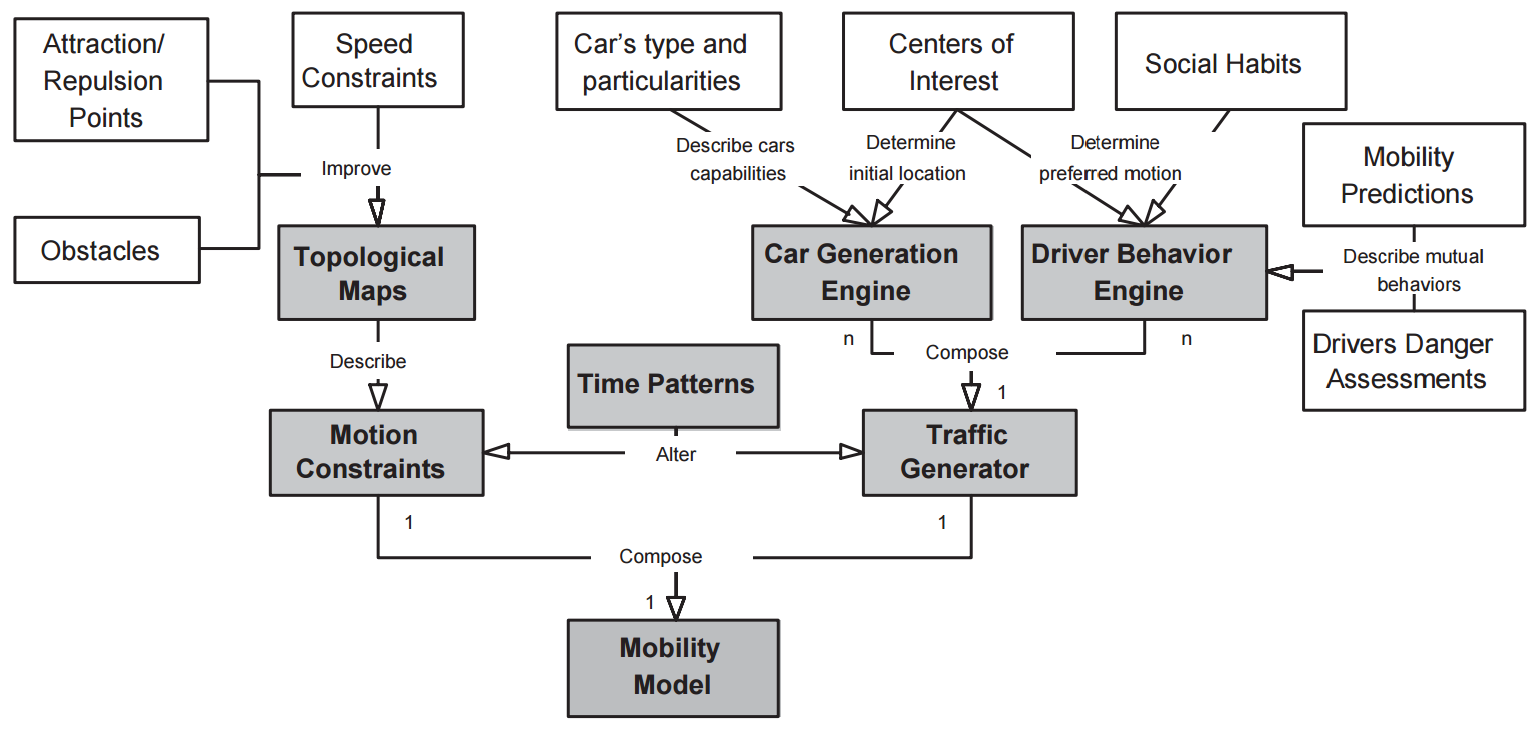
\includegraphics[width=8cm]{Prevision/Model/modelisation_simulation}
\centering
\caption{Cadre de travail pour des modèles réalisates de simulation routière - Source: \textit{Institut Eurécom}~\cite{harri2009mobility}}
\end{figure}

Nous l'avons dit, vérifier l'exactitude des simulateurs est une tâche peu aisée. Néanmoins, des études ont tenté de tester l'efficacité de ceux-ci en fournissant une cartographie entière de la région et en donnant le comportement macroscopique de la zone considérée~\cite{baumann2008generic} ou encore en comparant la simulation à des images prises d'un avion pour la ville de Porto, Portugal~\cite{ferreira2009stereoscopic}. A l'inverse, à un niveau microscopique, des capteurs ont été placés sur les routes afin de mieux comprendre le comportements des véhicules à l'instar des études sur Bologna, Italie~\cite{bieker2015traffic} ou sur le Luxembourg~\cite{pigne2011vehicular}. Le plus gros jeu de données est sans celui pour tout le canton de Zürich, Suisse qui correspond à l'ensemble des déplacements des véhicules pour une journée entière~\cite{raney2003agent}.

Cependant, les exemples précédents ont été générés en fournissant des données macroscopiques et microscopiques à un simulateur. Les trajets ont donc peut-être des comportements peu naturels et non représentatifs de l'activité réelle. Heureusement, il existe des exemples de déplacements réels tirés des réseaux de transport urbain ou de la circulation des taxis~\cite{yuan2010t}.

En vue d'obtenir une vision fort complète du trafic avec un haut niveau de granularité et ce sur une large région, une initiative appelée \textit{TAPASCologne}~\cite{TapasCologne} de l'\textit{Institute of Transportation Systems at the
German Aerospace Center} (ITS-DLR) vise à reproduire le plus fidèlement possible le trafic de véhicules dans la ville de Köln, Allegmane. Mais elle fait figure d'exception pour le moment.

\section{Données}

Un jeu de données qui a particulièrement retenu mon attention est lié à la ville de Aarhus, Danemark~\cite{CityPulseSmartCityDataset}. Celui-ci est une collections de données sur le trafic de véhicules, observés entre deux points pour une durée de plus de 6 mois (sur 449 points d'observations au total). Les données sont disponibles au format CSV et annoté au format des modèles d'information CityPulse. On peut également obtenir les informations en temps réel~\cite{CityPulseSmartCityDatasetRealTime}.

À chaque point d'observation est associé des méta-données qui donnent des informations sur le flux de données comme la position des senseurs, la distance entre-eux, le type de route, les précisions des capteurs, etc...

Chaque jeu de données est composée de plusieurs fichiers qui représentent les mesures effectuées entre deux capteurs. Dans ces fichiers, indexés par le temps par intervalle de 15 minutes, on retrouve le temps moyen, la vitesse moyenne et le nombre de véhicules ayant circulé entre ces points.

\section{Prévisions}

L'idée serait d'effectuer un travail analogue à celui de \textit{TAPASCologne} mais pour la ville d'Arrhus, Danemark. Cela consisterait tout d'abord à trouver une cartographie de la ville qui contiendrait une idée sur les lieux d'intérêts ainsi que toutes les rues (cf. Open Street Map~\cite{OpenStreepMap}) afin d'en extraire la topologie routière. Ce travail pourrait s'accompagner par une étude plus sociale sur la ville pour mieux comprendre les quartiers~\cite{OpenDataAarhus}. Ensuite, trouver des indications sur les problèmes de trafics dans cette ville et sur les demandes de déplacements des utilisateurs. Continuer par une simulation qui serait effectuée dans le logiciel SUMO en s'assurant que l'offre et la demande soit assurée (algorithme de Gawron~\cite{gawron1998iterative}).

La première étape consisterait à tester la cohérence des données et à vérifier qu'elles soient bien complètes. Il faudrait voir l'évolution du nombre de véhicules en train d'effectuer un trajet, en partance et à destination; ce qui donnerait des indications sur des signes de congestion excessive. Il y aurait alors sans doute du travail afin de corriger les comportements dans le but d'obtenir des résultats plus naturels (pics aux heures d'arrivées et de départs au travail, creux pendant la nuit, ...). Peut-être faudra-t-il penser à traiter des problèmes d'à-coups dans cette population et des informations inconsistantes sur les routes liées à des travaux. Tout cela s'effectuerait par le biais de diverses librairies écrites en R, on pense notamment à SpatioTemporal~\cite{keller2015unified} et spastat~\cite{baddeley2016spatial} qui offrent de nombreux outils dédiés à cette problématique.

Enfin, on serait en mesure de tester une simulation, de s'assurer que des comportements logiques et cohérents soient bien rendus. Pour pouvoir lancer des analyses plus générales et à larges échelles. A l'instar d'études précédentes sur la ville de Köln nottament~\cite{uppoor2011large, uppoor2012insights}. Et finalement comparer les résultats du simulateur avec ceux observés. Notons qu'il s'agit d'un jeu de données qui n'a été le sujet d'aucune étude pour le moment.